\documentclass{article}
\usepackage[a4paper, total={6.5in, 10in}]{geometry}
% \usepackage[english]{babel}
% \usepackage{graphicx}
% \usepackage[colorlinks=true, allcolors=black]{hyperref}
% \graphicspath{{img/}}
% \usepackage{amsmath}
%\usepackage{indentfirst}

% \usepackage{listings}
%\renewcommand{\lstlistingname}{Code}

% \usepackage{xcolor} 
% \definecolor{vgreen}{RGB}{104,180,104}
% \definecolor{vblue}{RGB}{49,49,255}
% \definecolor{vorange}{RGB}{255,143,102}
% \definecolor{vpurple}{RGB}{148,0,209}
% \definecolor{vgray}{RGB}{245,245,245}

% \lstdefinestyle{verilog-style}{
% 	backgroundcolor=\color{vgray},   
% 	commentstyle=\color{vgreen},
% 	keywordstyle=\color{vblue},
% 	numberstyle=\tiny\color{black},
% 	stringstyle=\color{vpurple},
% 	basicstyle=\scriptsize\small,
% 	breakatwhitespace=false,         
% 	breaklines=true,                 
% 	captionpos=t,                    
% 	keepspaces=true,                 
% 	numbers=left,                    
% 	numbersep=5pt,                  
% 	showspaces=false,                
% 	showstringspaces=false,
% 	showtabs=false,                  
% 	tabsize=3,
% 	language=Verilog,
% 	framesep=3mm
% }

\begin{document}
  %   \makeatletter
	% \renewcommand{\@seccntformat}[1]{}
	% \makeatother
	
  %   \clearpage
\setcounter{page}{1}

\begin{center}
    \vspace*{3em}
    {\LARGE \textbf{Machine Exercise 1}}\\
    {\vspace{1.5em}}
    {\large Vivado Familiarization}\\
\end{center}

\section{Introduction}
    hi
  %   \clearpage
\setcounter{page}{1}

\begin{center}
    \vspace*{3em}
    {\LARGE \textbf{Machine Exercise 2}}\\
    {\vspace{1.5em}}
    {\large Combinational Circuit I}\\
\end{center}

\section{Introduction}
    hi
  %   \clearpage
\setcounter{page}{1}

\begin{center}
    \vspace*{3em}
    {\LARGE \textbf{Machine Exercise 3}}\\
    {\vspace{1.5em}}
    {\large Combinational Circuit II}\\
\end{center}

\section{Introduction}
    hi
  %   \clearpage
\setcounter{page}{1}

\begin{center}
    \vspace*{3em}
    {\LARGE \textbf{Machine Exercise 4}}\\
    {\vspace{1.5em}}
    {\large Up-Down Counter}\\
\end{center}

\section{Introduction}
    hi
  %   \clearpage
\setcounter{page}{1}

\begin{center}
    \vspace*{3em}
    {\LARGE \textbf{Machine Exercise 5}}\\
    {\vspace{1.5em}}
    {\large Tri-Color LEDs}\\
\end{center}

\section{Introduction}
		hi
  %   \clearpage
\setcounter{page}{1}

\begin{center}
    \vspace*{3em}
    {\LARGE \textbf{Machine Exercise 6}}\\
    {\vspace{1.5em}}
    {\large Sequential Multiplication}\\
\end{center}

\section{Introduction}
    hi
  %   \clearpage
\setcounter{page}{1}

\begin{center}
    \vspace*{3em}
    {\LARGE \textbf{Machine Exercise 7}}\\
    {\vspace{1.5em}}
    {\large Vending Machine}\\
\end{center}

\section{Introduction}
    For this machine exercise, you will implement a state machine using Verilog.
		
	\section{Vending Machine}
		\begin{enumerate}
			\item Implement a vending machine that sells one type of item: item A which costs PHP 2. Your top-level module should be defined as follows:
			
\begin{lstlisting}[style={verilog-style}, caption={Module declaration of the vending machine.} , label={code:vendo}]
module vendo(
	clk, nrst,
	sel_A,
	p_1, p_5,
	disp_A,
	change
);

	input clk, nrst;
	input sel_A;
	input p_1, p_5;
	output disp_A;
	output change;

endmodule
\end{lstlisting} 

			\item The general behavior of the vending machine should be as follows:
				\begin{enumerate}
					\item The \texttt{clk} and \texttt{nrst} inputs serve as the clock and active-low reset, respectively. Asserting \texttt{nrst} (setting it to 0) should set the outputs \texttt{disp\_A} and \texttt{change} to 0. Otherwise, the machine will go to the starting state of the vending process.
					
					\item From a starting state, the user selects the item to be dispensed. This is done using the \texttt{sel\_A} input. If item A (PHP 2) is selected, the user sets \texttt{sel\_A} to 1 for a clock cycle. The other inputs (\texttt{p\_1}, \texttt{p\_5}) are ignored during this step.
					
					\item After selecting the item, the user inputs coins using the \texttt{p\_1} and \texttt{p\_5} inputs. The \texttt{p\_1} and \texttt{p\_5} inputs represent PHP 1 and PHP 5 coins, respectively. For a single coin to be inserted, the corresponding input should be set to 1 for a clock cycle. We place a restriction that only one of the two inputs (\texttt{p\_1}, \texttt{p\_5}) can be set to 1 during this step of the vending process. This step repeats until there is enough money inserted for the selected item. The other input (\texttt{sel\_A}) is ignored during this step.
					
					\item Once enough money has been inserted, the machine immediately dispenses the item. If the user selected item A, \texttt{disp\_A} should be set to 1 on the same clock cycle that the last coin has been inserted. It is only during this step that the \texttt{disp\_A} output can be set to 1. Otherwise, it is set to 0 by default. All inputs (\texttt{sel\_A}, \texttt{p\_1}, \texttt{p\_5}) are ignored during this step. If the money inserted was exactly the same as the item cost, the machine then proceeds back to the starting state. Otherwise, the machine proceeds to dispense change.
					
					\item The machine dispenses change in PHP 1 increments. This is represented by the output \texttt{change}. The machine starts to dispense change in the same clock cycle that the item is dispensed. A single clock cycle where the output \texttt{change} is set to 1 represents a dispensed PHP 1 coin. This step is repeated until all change has been dispensed. It is only during this step that the output \texttt{change} can be set to 1. Otherwise, it is set to 0 by default. All inputs (\texttt{sel\_A} \texttt{p\_1}, \texttt{p\_5}) are ignored during this step. After dispensing all of the change, the machine then proceeds back to the starting state.
					
				\end{enumerate}
			
			\item Design a testbench that implements the timing diagram shown in Figure \ref{fig:testbench}. An example response of the machine is also included in the timing diagram below. Verify the functionality of your design (not yet synthesized) using this testbench. 
				\begin{figure}[!htbp]
					\centering
					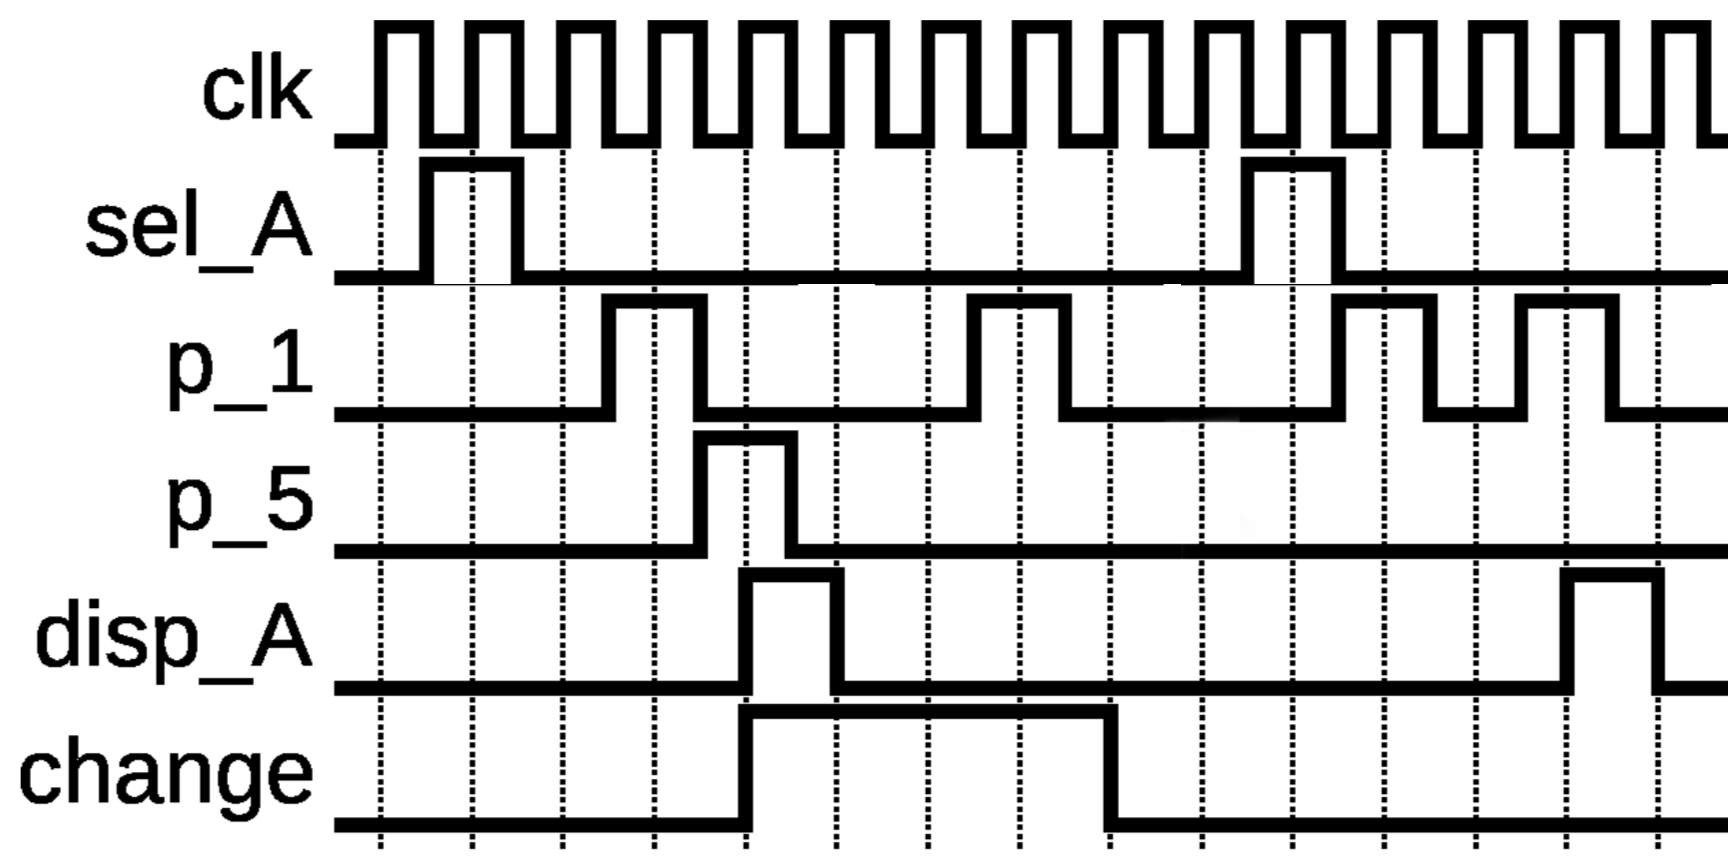
\includegraphics[width=0.55\textwidth]{me5_testbench}
					\caption{Vending machine testbench.}
					\label{fig:testbench}
				\end{figure}
			
			
			\item Implement your design on the Arty-7 35T Evaluation Kit board. Associate each port of your module to an FPGA pin as shown in the port mapping in Table \ref{tab:port}.
			
				\begin{table}[!htbp]
					\centering
					\caption{Port mapping.}
					\label{tab:port}
					\begin{tabular}{ | l | l | }
						\hline
						\multicolumn{1}{|c|}{Module Port} & \multicolumn{1}{c|}{FPGA Pin} \\
						\hline\hline
						\texttt{clk} & on-board $100MHz$ clock \\
						\hline
						\texttt{nrst} & SW0 \\
						\hline
						\texttt{sel\_A} BTN0 \\
						\hline
						\texttt{p\_1} & BTN1 \\
						\hline
						\texttt{p\_5} & BTN2 \\
						\hline
						\texttt{disp\_A} & LED1 \\
						\hline
						\texttt{change} & LED0 \\
						\hline
					\end{tabular}
				\end{table}
		\end{enumerate}
  %   \clearpage
\setcounter{page}{1}

\begin{center}
    \vspace*{3em}
    {\LARGE \textbf{Machine Problem}}\\
    {\vspace{1.5em}}
    {\large Tri-color LED PWM}\\
\end{center}

\section{Introduction}
    The intensity of the tri-color LEDs of the Artix-7\texttrademark{} 35T board can be controlled by varying its pulse width. This process of controlling the pulse width is called the pulse width modulation (PWM). For this project, you are tasked to make a PWM for the three colors of the LED, red, green, and blue depending on the value of the 8-bit input.

\section{Pulse Width Modulator}

\begin{enumerate}
    \item Implement the pulse width modulator. The top-level module should be defined as follows:
    
    \begin{lstlisting}[style={verilog-style}, caption={Code of \texttt{led\_pwm.v}} , label={code:pwm}]
module led_pwm(
	input clk,
	input nrst,
	input [3:0] nibble_in,
	input [2:0] sel,
	input acc,
	output [3:0] notif
);

endmodule
\end{lstlisting}

    \item Upon asserting \texttt{nrst} to 1, the notification output for 
    \item \texttt{nibble_in} is the input that will dictate the pulse width of each of the colors. To completely send the 8-bit input, 
\end{enumerate}

\section{LED Driver}

\begin{enumerate}
    \item Implement the LED driver. This will accept an 8-bit input and outputs a corresponding signal for the LED with a duration dictated by the input. Save this as "\texttt{led\_driver.v}".
    
    \begin{lstlisting}[style={verilog-style}, caption={Code of \texttt{led\_driver.v}} , label={code:driver}]
module led_driver(
	input clk,
	input nrst,
	input [7:0] pw,
	input [2:0] rgb_sel,
	input en,
	output [2:0] rgb_drv
);

    localparam [16:0] maxtick = 100000; // Ticks in 1 ms
    
    reg [16:0] max_pw_r_count, max_pw_g_count, max_pw_b_count;
    reg [16:0] r_high_count, g_high_count, b_high_count;
    reg [16:0] r_low_count, g_low_count, b_low_count;
    reg r_high_en, g_high_en, b_high_en;

    // Set maximum tick counts    
    always@(posedge clk or negedge nrst)
        if(!nrst)
            begin
                max_pw_r_count <= 17'd0;
                max_pw_g_count <= 17'd0;
                max_pw_b_count <= 17'd0;
            end
        else
            case({rgb_sel, en})
                4'd8:
                    begin
                        max_pw_r_count <= 17'd197 * {9'd0, pw};
                        max_pw_g_count <= max_pw_g_count;
                        max_pw_b_count <= max_pw_b_count;
                    end
                4'd4:
                    begin
                        max_pw_r_count <= max_pw_r_count;
                        max_pw_g_count <= 17'd197 * {9'd0, pw};
                        max_pw_b_count <= max_pw_b_count;
                    end
                4'd2:
                    begin
                        max_pw_r_count <= max_pw_r_count;
                        max_pw_g_count <= max_pw_g_count;
                        max_pw_b_count <= 17'd197 * {9'd0, pw};
                    end
                default:
                    begin
                        max_pw_r_count <= max_pw_r_count;
                        max_pw_g_count <= max_pw_g_count;
                        max_pw_b_count <= max_pw_b_count;
                    end
            endcase
    
    // HIGH pulse tick counter
    always@(posedge clk or negedge nrst)
        if(!nrst)
            begin
                r_high_count <= 17'd0;
                g_high_count <= 17'd0;
                b_high_count <= 17'd0;
            end
        else
            if(en)
                begin
                    if((r_high_count < max_pw_r_count) && (r_high_en == 1))
                        r_high_count <= r_high_count + 17'd1;
                    else
                        r_high_count <= 17'd0;
                    if((g_high_count < max_pw_g_count) && (g_high_en == 1))
                        g_high_count <= g_high_count + 17'd1;
                    else
                        g_high_count <= 17'd0;
                    if((b_high_count < max_pw_b_count) && (b_high_en == 1))
                        b_high_count <= b_high_count + 17'd1;
                    else
                        b_high_count <= 17'd0;
                end
            else
                begin
                    r_high_count <= 17'd0;
                    g_high_count <= 17'd0;
                    b_high_count <= 17'd0;
                end

    // LOW pulse tick counter
    always@(posedge clk or negedge nrst)
        if(!nrst)
            begin
                r_low_count <= 17'd0;
                g_low_count <= 17'd0;
                b_low_count <= 17'd0;
            end
        else
            if(en)
                begin
                    if((r_low_count < (maxtick - max_pw_r_count)) && (r_high_en == 0))
                        r_low_count <= r_low_count + 17'd1;
                    else
                        r_low_count <= 17'd0;
                    if((g_low_count < (maxtick - max_pw_g_count)) && (g_high_en == 0))
                        g_low_count <= g_low_count + 17'd1;
                    else
                        g_low_count <= 17'd0;
                    if((b_low_count < (maxtick - max_pw_b_count)) && (b_high_en == 0))
                        b_low_count <= b_low_count + 17'd1;
                    else
                        b_low_count <= 17'd0;
                end
            else
                begin
                    r_low_count <= 17'd0;
                    g_low_count <= 17'd0;
                    b_low_count <= 17'd0;
                end

    // HIGH and LOW pulse tick counter enabler
    always@(*)
        begin
            if(r_high_count == max_pw_r_count)
                r_high_en = 0;
            else
                r_high_en = 1;
            if(g_high_count == max_pw_g_count)
                g_high_en = 0;
            else
                g_high_en = 1;
            if(b_high_count == max_pw_b_count)
                b_high_en = 0;
            else
                b_high_en = 1;
        end

    assign rgb_drv[2] = en & r_high_en;
    assign rgb_drv[1] = en & g_high_en;
    assign rgb_drv[0] = en & b_high_en;

endmodule
\end{lstlisting}
    
    \item The 8-bit input \texttt{pw} is the input to the driver. All possible values of \texttt{pw} maps from 0\% to 50\% duty ccyle.
    
    \item The bus \texttt{rgb\_sel} selects between the red, green, and blue light components of the LED. This is used to specify which color you are currently setting up. Asserting \texttt{rgb\_sel[2]} to 1 selects red, asserting \texttt{rgb\_sel[1]} to 1 selects green, and asserting \texttt{rgb\_sel[0]} to 1 selects blue. Other values for \texttt{rgb\_sel} will do nothing.
    
    \item Asserting \texttt{en} to 1 starts the modulator by the use of counters. The modulator will start to produce the outputs necessary to drive the tri-color LED. The values of the pulse width can no longer be changed during this time (i.e.: when \texttt{en} = 1).
    
    \item The output is \texttt{rgb\_drv}. The red color driver is at \texttt{rgb\_drv[2]}, blue at \texttt{rgb\_drv[1]}, and the green driver is at \texttt{rgb\_drv[0]}.

\end{enumerate}

\end{document}